\documentclass[twocolumn,onesided,9pt]{article}

\usepackage{./Task32FlyerLatexStyle/Task32Flyer}
\usepackage{todonotes}
\usepackage{ragged2e}
%% -----------------------------------
%% Document information
%% -----------------------------------
\def\pubdate{26 June 2020}
\shorttitle{Webinar summary}
\doctype{IEA Wind Task 32 webinar summary}
\title{Approaches in filtering data from pulsed wind lidar}
\DOI{10.5281/zenodo.3909488}
\version{}
\addbibresource{bibliography.bib}

\newcommand{\orcid}[1]{\href{https://orcid.org/#1}{
\includegraphics[width=8pt]{graphics/ORCIDiD_icon128x128.png}}}
\usepackage{fontawesome}
\newcommand{\mailme}[1]{\href{mailto:#1}{\faicon{envelope-o}}}

%% ===================================
%% Document starts
%% ===================================

\begin{document}

%% -----------------------------------
%% Title
%% -----------------------------------
\maketitle
\thispagestyle{cover}

%%
%% Authors
%% 
\noindent\begin{minipage}{\columnwidth}
\textcolor{TextLightGrey}{Authors: Leonardo Alcayaga~\orcid{0000-0003-4175-9024},
Rogier Floors~\orcid{0000-0002-9363-4699},
Pedro Santos~\orcid{0000-0003-2962-1364}. Editor: Andrew Clifton~\orcid{0000-0001-9698-5083}}~\mailme{clifton@ifb.uni-stuttgart.de}%
\end{minipage}
\vskip 6pt

%% -----------------------------------
%% Teaser text
%% -----------------------------------
{\Large\noindent\nohyphens\raggedright{%
Can more of a pulsed wind lidar's output data be used to get more accurate results and increased coverage?%
}}
\vskip 6pt

\begin{tcolorbox}[colback=Task32Blue2,
                    coltext=White,
                    colframe=Task32Blue2,
                    boxsep=0pt,
                    left=3pt,
                    right=3pt,
                    top=3pt,
                    bottom=3pt,
                    center,
                    valign=top,
                    halign=left]
 
     This is a summary of the ``Filtering lidar data'' webinar given by Rogier Floors and Leonardo Alcayaga on 7 April 2020 in the IEA Wind Task 32 webinar series. It represents the authors' opinions.
  \end{tcolorbox}


%% -----------------------------------
%% Introductory text
%% -----------------------------------
Wind lidar and other wind measurement devices often report a range of data metrics in the output files. It is sometimes tempting to use these data as filters.

One metric often used for filtering is the Carrier-to-noise ratio (CNR). The CNR of a pulsed lidar indicates the relative strength of the signal versus background noise. It depends, among other things, on the backscatter properties of the atmosphere, the range, and the strength of the laser used in the lidar device \citep{Aitken_2012_a}.  Therefore, care must be taken to select appropriate CNR levels and not systematically exclude data.

This paper has two main threads. Firstly, the authors outline the effect of data selection on the wind climatology using ground-based profiling pulsed lidars, and how this might be mitigated. And, they present a way to achieve better spatial coverage by applying a filtering algorithm that uses several metrics.

%% -----------------------------------
%% Wind climatology from profiling lidar - Rogier & Sven-Erik
%% -----------------------------------

\section*{How to determine wind climatology from profiling lidar} % Rogier & Sven-Erik

Wind climatologies are sensitive to data availability. Therefore the choice of CNR threshold for 10-minute mean wind speeds can impact the wind climatology. 

Data collected at the FINO3 platform in the North Sea  was recently used to quantify this effect \cite{Gryning_Floors_CNR}. When the Carrier-to-Noise-Ratio (CNR) threshold value is increased, the wind speed distribution is shifted to higher values (Fig. \ref{fig:CNR_sensitivity}).

\begin{figure}[ht]
    \centering
    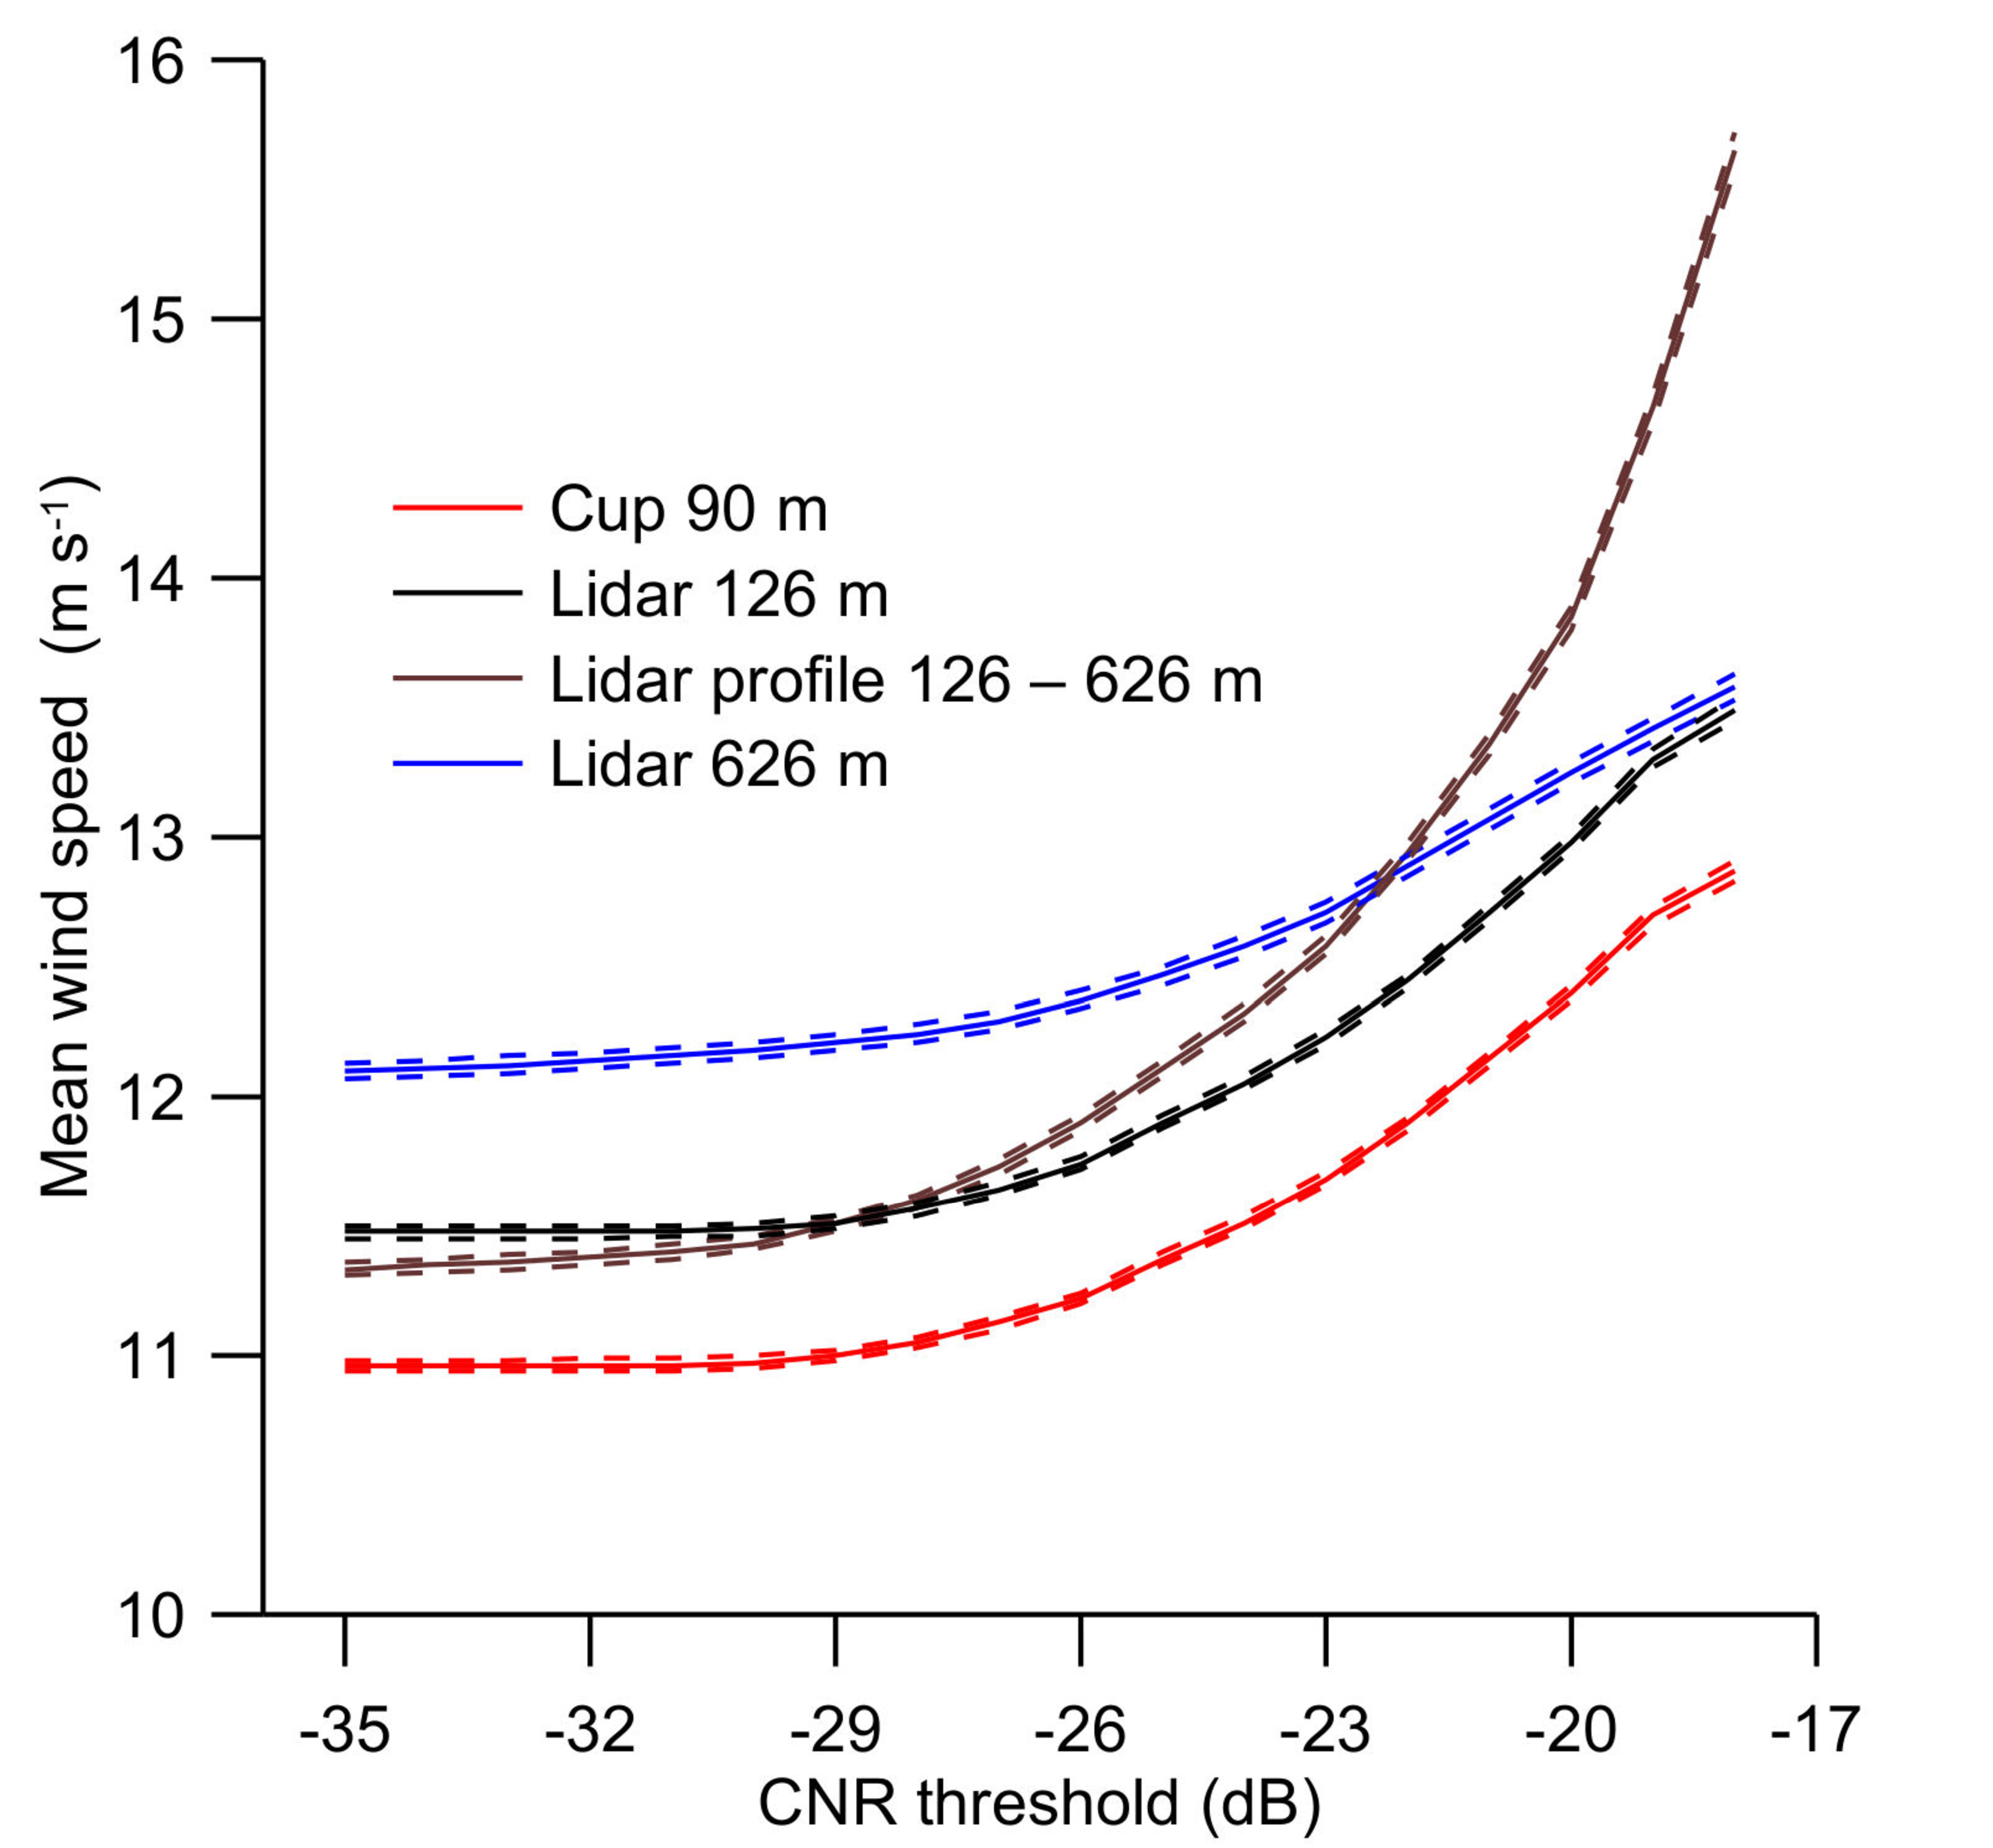
\includegraphics[trim=12pt 12pt 12pt 12pt, clip, width=\columnwidth]{fig/figure.pdf}
    \caption{The effect of lidar CNR limits on the observed wind climatology at the FINO 3 platform. Data are for one year. The standard error is shown by dashed lines.}
    \label{fig:CNR_sensitivity}
\end{figure}

The factory setting of the CNR threshold for this long-range lidar was -35 dB. The data availability from this CNR threshold gives the lowest annual mean wind speed estimate using the range gate at 126 m. The mean wind speed increases to $\approx$13 m s$^{-1}$ when the filtering threshold is set to -17 dB. The mean wind speed from the cup anemometer measured at 90 m shows a very similar increase, showing that the bias is not induced by the lidar, but is a consequence of \textbf{data availability}. Finally, filtering by requiring that data exceed a CNR threshold at all range gates from 126 to 626 m results in an even stronger effect, because data that fulfill this criterion at all heights are rare.

This effect of CNR threshold on data was also observed for both short- and long-range vertical profilers and for scanning lidars (see Fig. 10 in \cite{Gryning_Floors_CNR} or the webinar presentation \cite{rogier_floors_2020_3743076} for more examples). The effects described here are hard to detect from e.g. a scatter plot comparison between a lidar and a met mast mounted cup anemometer: there may be a perfect correlation between the two, but the climatological wind speed at the same location can still be different when the measurements do not cover 100\% of the period. This is because lower CNR values apparently correlate with lower wind speeds. The physical mechanism for this correlation was not investigated, but it was present in data collected in Germany, Denmark, and Greenland.

For more information see the webinar presentation \citep{rogier_floors_2020_3743076} or the publication \cite{Gryning_Floors_CNR}.

%% -----------------------------------
%% Scanning data filtering - Leonardo?
%% -----------------------------------
% Why go beyond CNR filtering?
\section*{Increasing spatial coverage}

Long-range pulsed lidars tend to show lower CNR values at longer ranges. So, using CNR as a filter would reduce availability with increasing range. This can reduce the spatial coverage of scanning lidars. 

But, this filtering may be unreasonably reducing data availability. For example, the distribution of the line-of-sight wind speed ($V_{LOS}$) in Figure~\ref{fig:CNR_Vlos_range} shows apparently reasonable values, even for low CNR.

\begin{figure}[ht]
    \centering
    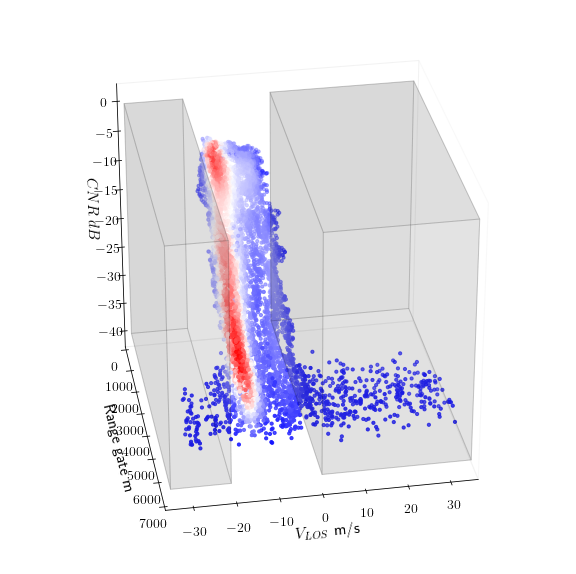
\includegraphics[trim=36pt 30pt 36pt 36pt, clip,width=\columnwidth]{fig/CNR_Vlos_range.png}
    \caption{Sometimes low-CNR data at longer ranges still have reasonable $V_{LOS}$ values. These data can be lost if a CNR threshold is used. (Colours indicates data density; red areas have more data than blue)}
    \label{fig:CNR_Vlos_range}
\end{figure}

What other quality indicators could be used?

One useful indicator is the \textbf{smoothness of the line-of-sight wind speed}; a good $V_{LOS}$ field should be continuous in the spatial domain. Therefore, a median filter can be used to detect ``bad'' data \citep{Menke_median_filter}. This is fast and efficient when the proper moving median window and filtering threshold are selected.

Another indicator is \textbf{data self-similarity}. Lidar data can be thought of as multi-dimensional data sets~--~described by e.g., spatial location, CNR, and wind speed~--~where reliable measurements cluster together \cite{Beck2017}. These clusters become clearer as more dimensions are included, and can be detected using a clustering algorithm like DBSCAN \cite{Ester1996}. DBSCAN detects coherent groups of data of arbitrary shape, separating them from the sparse observations associated with ``noisy data''. Selecting relevant data features in DBSCAN increases the data availability \cite{Alcayaga_DBSCAN} and the spatial coverage (Fig.~\ref{fig:CNR_Vlos_range_scan}). The DBSCAN classification parameters adjust automatically and so there is no need to define a threshold for any feature.

\begin{figure}[h]
\centering
\begin{subfigure}{\columnwidth}
  \centering
  % include first image
  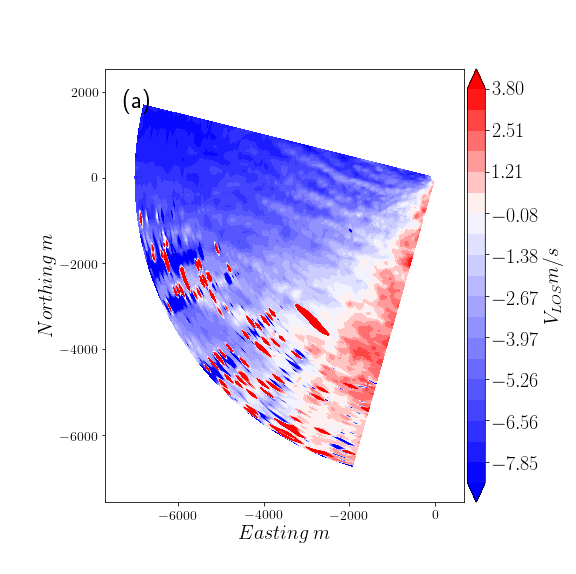
\includegraphics[trim=24pt 24pt 12pt 24pt, clip,width=\columnwidth]{fig/rawscan0.png}  
  \caption{The unfiltered scan data includes noisy data at farther ranges. The red and blue blobs are extreme values and indicate regions of noisy data.}
  \label{fig:CNR_Vlos_range_scan_raw}
\end{subfigure}
\begin{subfigure}{\columnwidth}
  \centering
  % include first image
  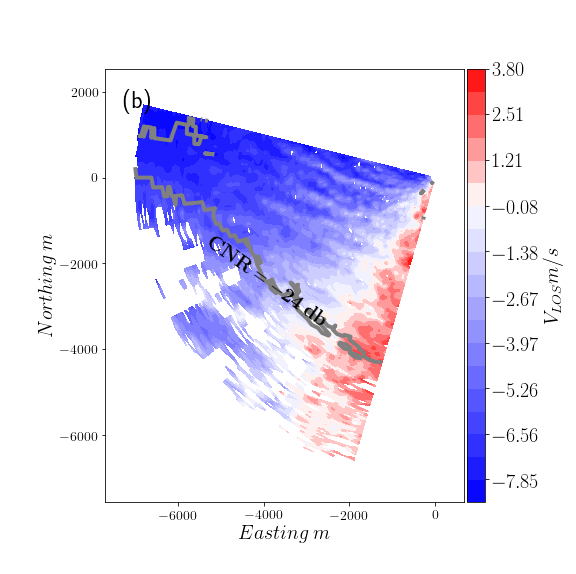
\includegraphics[trim=24pt 24pt 12pt 24pt, clip,width=\columnwidth]{fig/filtscan0.png}  
  \caption{The choice of filter can impact coverage. The background data has been filtered using DBSCAN. The grey contour shows the furthest range achieved using a CNR threshold of -24db.}
  \label{fig:CNR_Vlos_range_scan_filtered}
\end{subfigure}
    \caption{Filtering strategies affect spatial coverage.}
    \label{fig:CNR_Vlos_range_scan}
\end{figure}

For more information see the webinar presentation \citep{leonardo_alcayaga_2020_3742961}, or the related publication \cite{Alcayaga_DBSCAN}.

\clearpage

%% -----------------------------------
%% Summary
%% -----------------------------------
\section*{Summary and Implementation}
To minimize the impacts of the effect of threshold filtering on the mean wind speed, one needs to achieve a data availability that is as high as possible. How this can be done depends on your goals:
\begin{itemize}
    \item \textbf{when interested in winds at hub height} don't include measurement from heights above that, as the CNR tends to decrease with range and also the number of aerosols tends to decrease with height, thereby decreasing the data recovery rate.
    \item \textbf{when interested in wind shear} make sure to have a high ($>$95\%) and similar availability at all heights, because the filtered mean wind speed depends on data availability which generally decreases with height (Fig. \ref{fig:CNR_sensitivity}).
    \item \textbf{When availability is decreased by filtering} with a higher CNR threshold, compare the mean wind speed at the same range gate before and after the filtering to make sure they are similar.
\end{itemize}

To maximize the spatial coverage and data quality of retrievals from scanning lidars, one needs to go beyond CNR as the only quality parameter. Instead, $V_{LOS}$ and spatial information, and filtering techniques of increasing complexity can be used. When using these techniques, consider the following:
\begin{itemize}
    \item \textbf{First use a simpler and faster approach} based on smoothness, such as a median-like filter on $V_{LOS}$.
    \item \textbf{Check the statistics of the recovered data}. This could include comparing the distribution of $V_{LOS}$ against high CNR data (particularly the tails).
    \item The moving-median window size and threshold values used in median \textbf{filters must be tuned}.
    \item \textbf{If the results are not satisfactory} (e.g., tails in the distribution of $V_{LOS}$ are still heavier compared to high CNR data, there is evidence of noise, or changes in atmospheric conditions requires constant tuning of filter parameters), then a classification/clustering method based on data density may help. 
\end{itemize}

\vfill

%% -----------------------------------
%% References
%% -----------------------------------
%\section*{References}
% bibliography

% need accompanying information about Rogier's and Leonardo's presentations:
\defbibnote{webinar}{The presentations accompanying this paper are available through Zenodo \citep{rogier_floors_2020_3743076, leonardo_alcayaga_2020_3742961}.}
\label{sec:References}
\addcontentsline{toc}{section}{References}
{\small
\printbibliography[prenote=webinar]
}

\vfill


%% -----------------------------------
%% Outlined block of smaller text
%% -----------------------------------
\begin{tcolorbox}[width=1.0\columnwidth,
                  boxsep=0pt,
                  left=3pt,
                  right=3pt,
                  top=3pt,
                  arc=0pt,
                  boxrule=0.5pt,
                  toprule=0.5pt,
                  colback=white,
                  coltext=TextGrey
                  ]
{\footnotesize
This webinar summary was published by IEA Wind Task 32 to accompany a webinar that took place on 7 April 2020. The information presented here is the opinion of the authors.

%% -----------------------------------
%% IEA WIND AND TASK 32
%% -----------------------------------
\begin{tabular}{m{0.3\columnwidth}m{0.6\columnwidth}}
    % IEA Wind * DO NOT EDIT THIS TEXT *
    
\includegraphics[height=2cm]{graphics/IEAWind_logo.jpg} &
    The International Energy Agency is an autonomous organisation which works to ensure reliable, affordable and clean energy for its 30 member countries and beyond. The IEA Wind Technology Collaboration Programme supports the work of 38 independent, international groups of experts that enable governments and industries from around the world to lead programmes and projects on a wide range of energy technologies and related issues.  %
    \\
    % Task 32 * DO NOT EDIT THIS TEXT *
    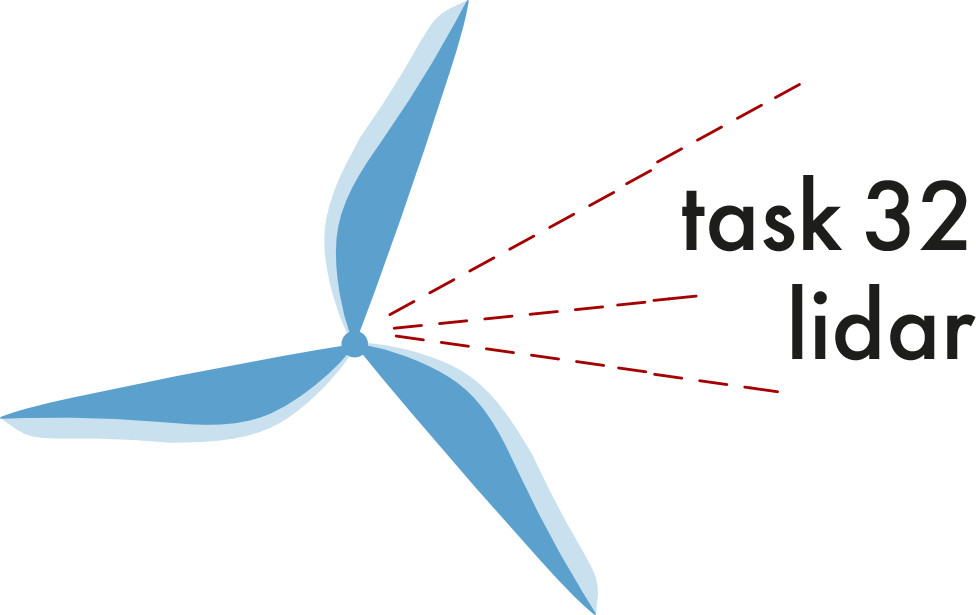
\includegraphics[height=1.5cm]{graphics/Task32_logo.jpg} &
    \href{www.ieawindtask32.org}{IEA Wind Task 32} exists to identify and mitigate the barriers to the deployment of wind lidar for wind energy applications.
\end{tabular}%

%% -----------------------------------
%% Authors
%% -----------------------------------
\textbf{Authors (alphabetical by family name):} %
Leonardo Alcayaga (DTU Wind Energy, Denmark)\orcid{0000-0003-4175-9024},
Rogier Floors (DTU Wind Energy, Denmark)\orcid{0000-0002-9363-4699},
Pedro Santos (DTU Wind Energy, Denmark)\orcid{0000-0003-2962-1364}.
\textbf{Editor:} Andrew Clifton (U. Stuttgart, Germany)\orcid{0000-0001-9698-5083}. %

%% -----------------------------------
%% Images
%% -----------------------------------
\textbf{Images:}
Banner, left to right: \href{https://unsplash.com/@alexkixa}{Alexandre Debiève on Unsplash}, \href{http://ifb.uni-stuttgart.de}{SWE U. Stuttgart}, \href{https://unsplash.com/@markusspiske}{Markus Spiske on Unsplash}. Figure 1 by R. Floors, Figure 2, 3 by L. Alcayaga.
}

%% -----------------------------------
%% End of highlighted block
%% -----------------------------------
\end{tcolorbox}

\end{document}
